\section{The Dependence of the Beam Coupling Impedance on The Kicker Components}

As part of the study to improve the beam screen it was decided to investigate systematically the effect of the various commponents of the kicker magnet on the resulting beam coupling impedance. This is divided into two sections, the study of the effect of the beam screen on the beam coupling impedance of the ferrite yoke, and subsequently a study of the effects of the dimensions of the beam screen and screen conductors on the beam coupling impedance.

\subsection{The Impedance of the MKI - Effects of the Inclusion of the Beam Screen}

To first judge the effectiveness of the concept of the beam screen as an impedance reduction technique we simulate the MKI by systematically adding components to the magnet to determine their effect on the beam coupling impedance. We consider the following configurations of the MKI:

\begin{enumerate}
\item{The c-core ferrite yoke}
\item{The c-core ferrite yoke with a ceramic cylinder inserted inside}
\item{As above but with 24 screen conductors inserted into the cylinder, capactively coupled at one end}
\item{The internal magnet structure including the vacuum tank, HV and ground plates and the surrounding connections.}
\end{enumerate}

These geometries are shown in Fig.~\ref{fig:mki-layout-buildup}, and the resulting impedance simulations for the real component shown in Fig.~\ref{fig:mki-buildup-impedance}. Several points can be seen; firstly that the inclusion of the beam screen with screen conductors very effectively screens the beam from the other components of the kicker magnet - including the ceramic of the beam screen, the surrounding structures and the ferrite itself. This indicates that for a beam screen in which the ceramic tube holds a large number of screen conductors, the beam is effectively screened from the surrounding structure up to a frequency characterised by seperation of the screen conductors. This has benefits for the impedance simulations as it is valid to use a reduced simulation model considering just the capacitively coupled end provided we can assume the ferrite is well screened (i.e. we have 24 screen conductors in place). Secondly the inclusion of the ceramic beam pipe does not effectively screen the ferrite by itself - the screen conductors are necessary to correctly screen the surroundings. And lastly that the use of the ceramic beam screen contributes significantly to the imaginary component of the longitudinal impedance (evidenced by the linear increase of the imaginary impedance with frequency due to the inductive component of the impedance) even with the presence of screen conductors.
 
\begin{figure}
\subfigure[]{
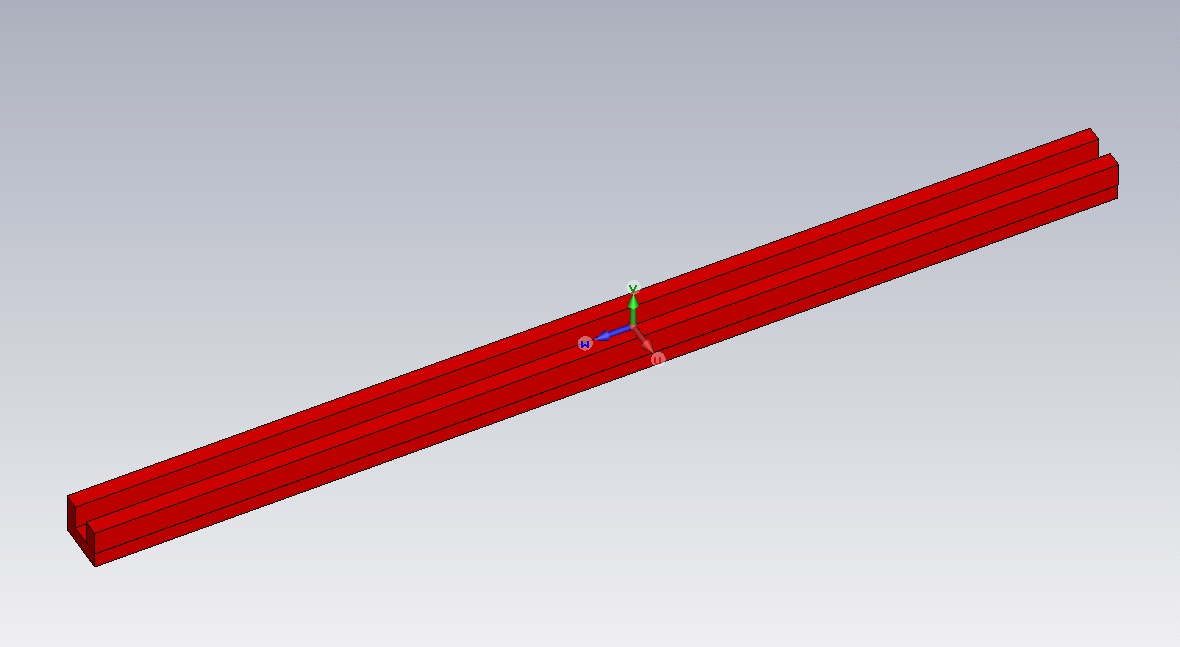
\includegraphics[width=0.45\textwidth]{LHC_MKI/figures/mki-buildup-ferrite.png}
\label{fig:mki-buildup-ferrite}
}
\subfigure[]{
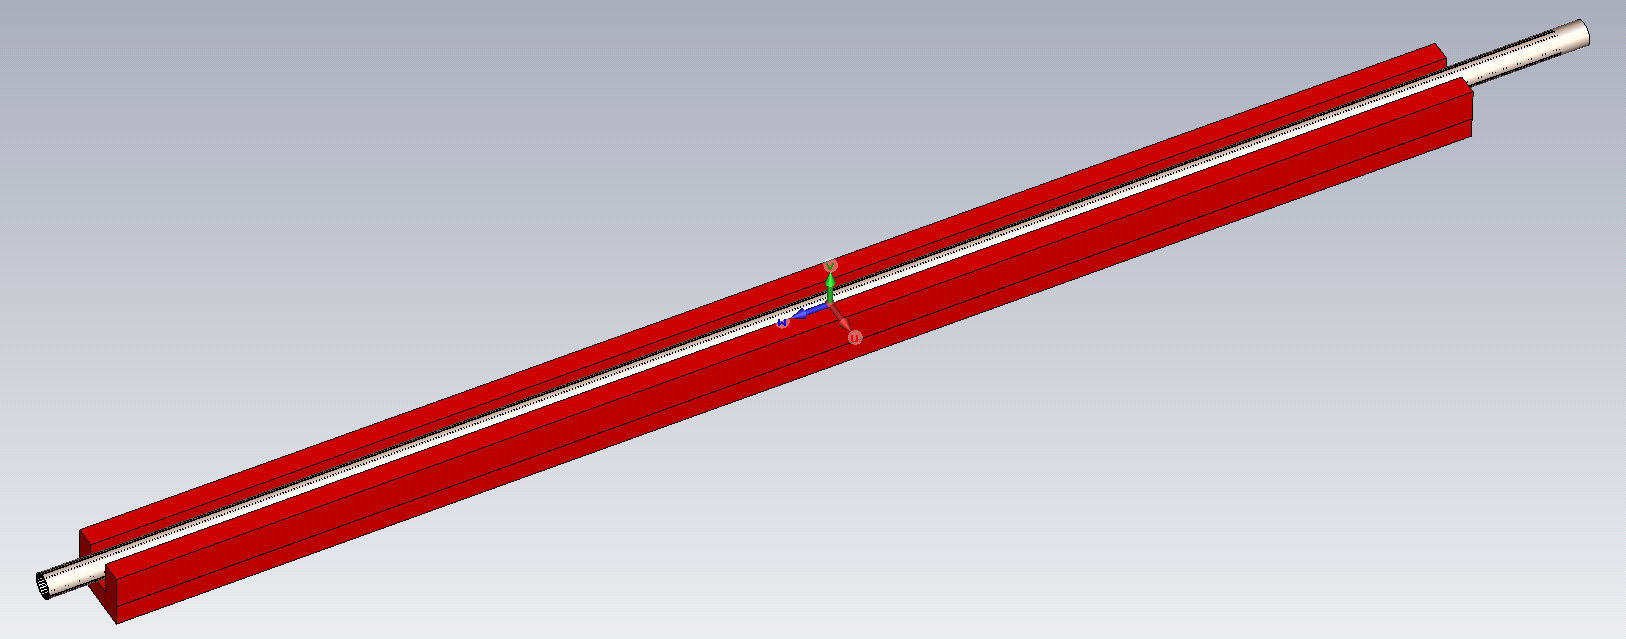
\includegraphics[width=0.45\textwidth]{LHC_MKI/figures/mki-buildup-ferrite-ceramic.png}
\label{fig:mki-buildup-ferrite-ceramic}
}
\subfigure[]{
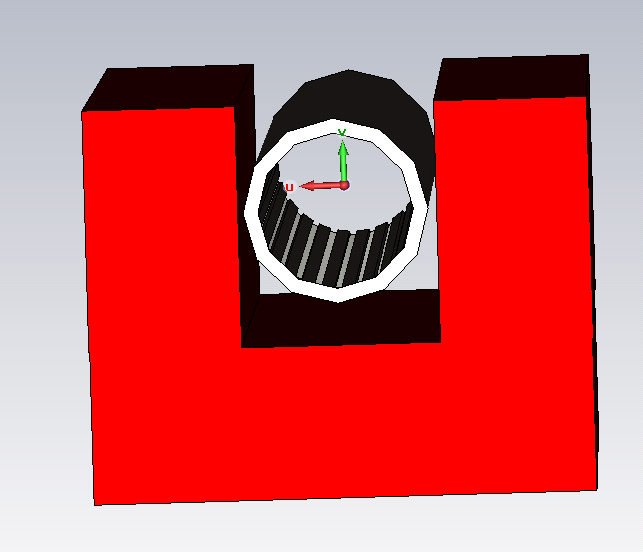
\includegraphics[width=0.45\textwidth]{LHC_MKI/figures/mki-buildup-ferrite-ceramic-cond.png}
\label{fig:mki-buildup-ferrite-ceramic-cond}
}
\subfigure[]{
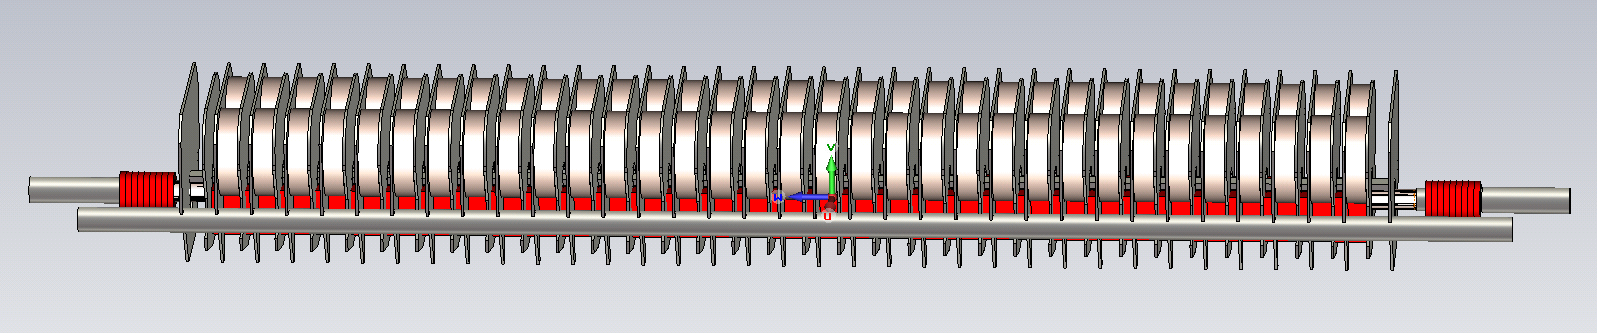
\includegraphics[width=0.45\textwidth]{LHC_MKI/figures/mki-buildup-ferrite-ceramic-cond-full.png}
\label{fig:mki-buildup-ferrite-ceramic-cond-full}
}
\label{fig:mki-layout-buildup}
\caption{The geometries simulated for the various components in the LHC-MKI. These are ferrite only \ref{fig:mki-buildup-ferrite}, ferrite and the ceramic beam screen \ref{fig:mki-buildup-ferrite-ceramic}, ferrite with the beam screen containing 24 screen conductors \ref{fig:mki-buildup-ferrite-ceramic-cond} and finally the complete MKI magnet \ref{fig:mki-buildup-ferrite-ceramic-cond-full}.}
\end{figure}

\begin{figure}
\subfigure[]{
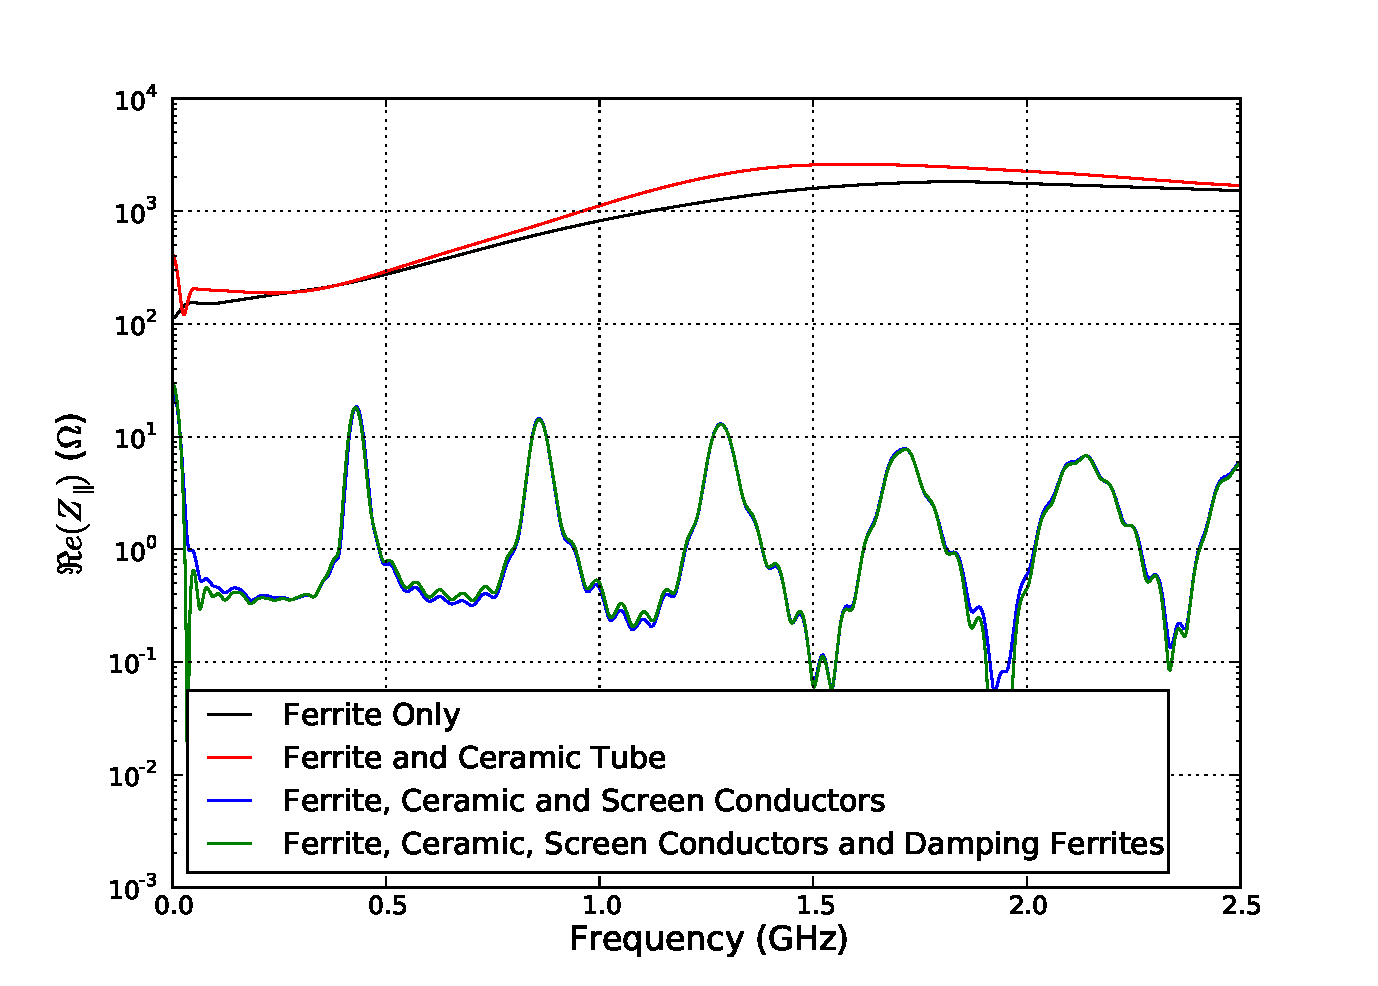
\includegraphics[width=0.5\textwidth]{LHC_MKI/figures/mki-build-up-real-imp.pdf}
\label{fig:mki-buildup-real-imp}
}
\subfigure[]{
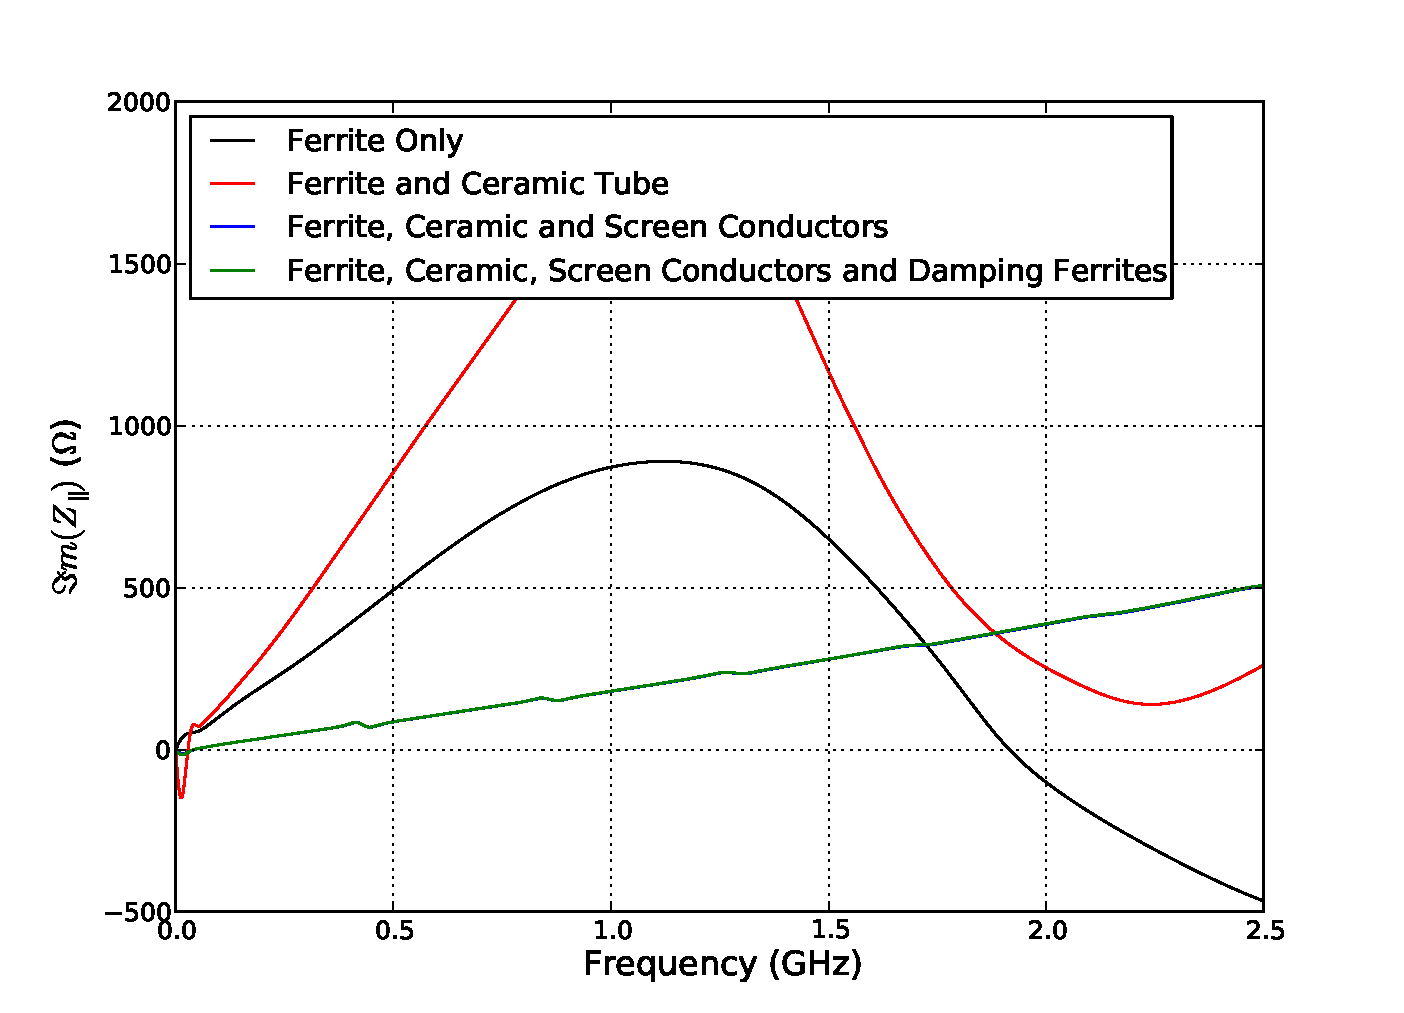
\includegraphics[width=0.5\textwidth]{LHC_MKI/figures/mki-build-up-imag-imp.pdf}
\label{fig:mki-buildup-imag-imp}
}
\label{fig:mki-buildup-impedance}
\caption{The \ref{fig:mki-buildup-real-imp} real component and the \ref{fig:mki-buildup-imag-imp} imaginary components of the LHC MKI kicker magnet impedances for different quantities of components in the magnet.}
\end{figure}


Concerning the role of the beam screen layout there are two areas to examine - the effect of different quantities of screening of the beam by having more or less screen conductors (in this case removing those directed towards the HV busbar as is likely due to concerns of electrical breakdown) and of the effect of different dimensions of the screen at the capacitively coupled end of the beam screen.

\subsection{How Screening Changes with the Number of Screen Conductors}

For the changes on the number of screen conductors two variations are carried out - The first is to examine the case of removing several screen conductors in the beam screen towards the HV busbar (shown in Fig.~\ref{fig:mki-take-away-cond-together}). This direction is chosen as these screen conductors experience the highest induced voltage during the firing of the kicker magnet, and additionally it was initially thought that on this side the HV busbar would provide some screening of the beam from the ferrite yoke. The second variation is to remove a selection of screen conductors towards the HV busbar (shown in Fig.~\ref{fig:mki-take-away-cond-alt}), in this case to examine whether it is possible to acquire some shielding through using some screen conductors and benefitting from removing some screen conductors to remove the rate of electrical breakdown.

\begin{figure}
\subfigure[]{
\label{fig:15-cond-together}
}
\subfigure[]{
\label{fig:19-cond-together}
}
\subfigure[]{
\label{fig:24-cond-together}
}
\label{fig:mki-take-away-cond-together}
\caption{Beam screens with different numbers of screen conductors removed from the design quantity of 24. Models of 15 \ref {fig:15-cond-together}, 19 \ref{fig:19-cond-together} and 24 \ref{fig:24-cond-together} screen conductors are considered for the impedance simulations. Conductors surrounded by the boxes are removed in this case.}
\end{figure}

\begin{figure}
\subfigure[]{
\label{fig:17-cond-alt}
}
\subfigure[]{
\label{fig:19-cond-alt}
}
\subfigure[]{
\label{fig:20-cond-alt}
}
\subfigure[]{
\label{fig:24-cond-alt}
}
\label{fig:mki-take-away-cond-ql5}
\caption{Beam screens with different numbers of screen conductors removed from the design quantity of 24. Models of 17 \ref {fig:17-cond-alt}, 19 \ref{fig:19-cond-alt}, 20 \ref{fig:20-cond-alt} and 24 \ref{fig:24-cond-alt} screen conductors are considered for the impedance simulations. Conductors that are coloured red are the removed in each case.}
\end{figure}

\begin{figure}
\subfigure[]{
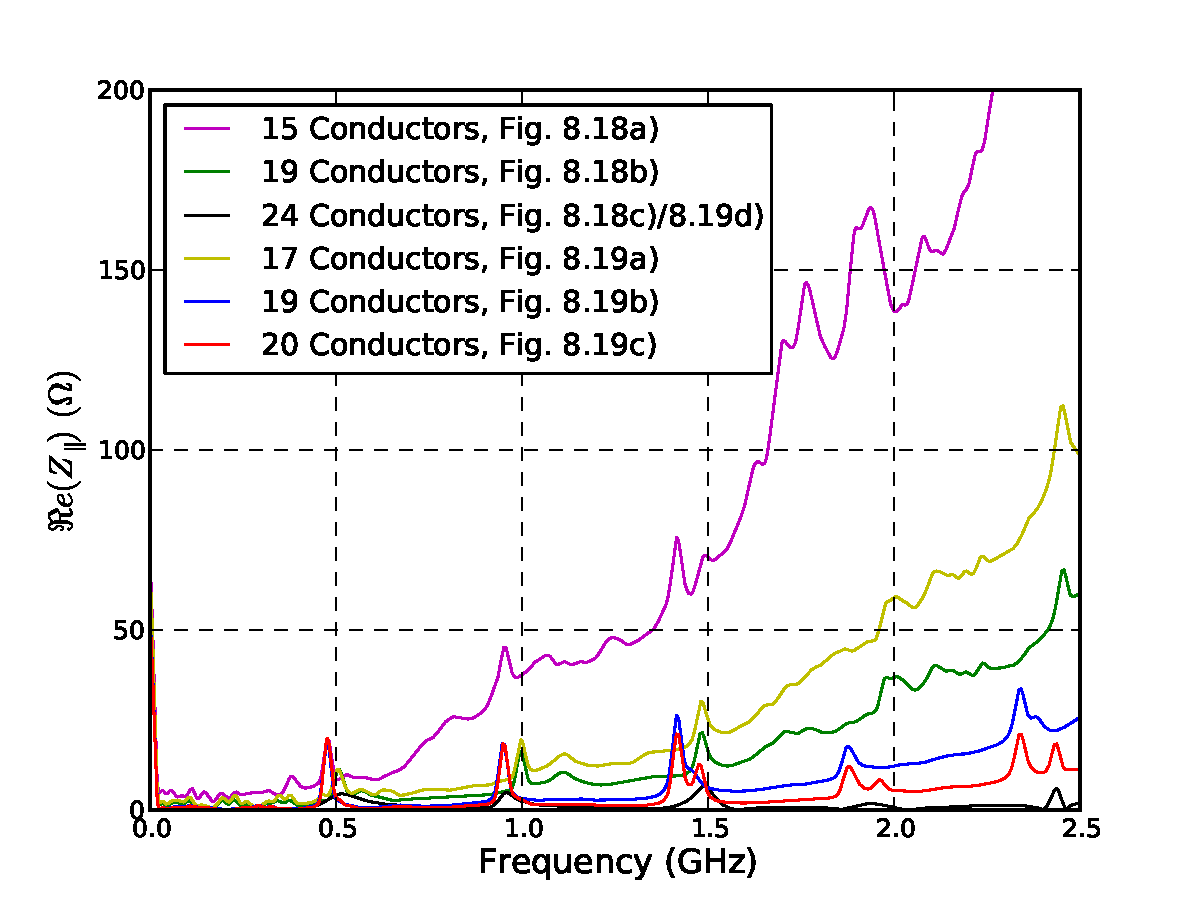
\includegraphics[width=0.5\textwidth]{LHC_MKI/figures/mki-no-screen-conductors-real-impedance.pdf}
\label{fig:remove-cond-real-imp}
}
\subfigure[]{
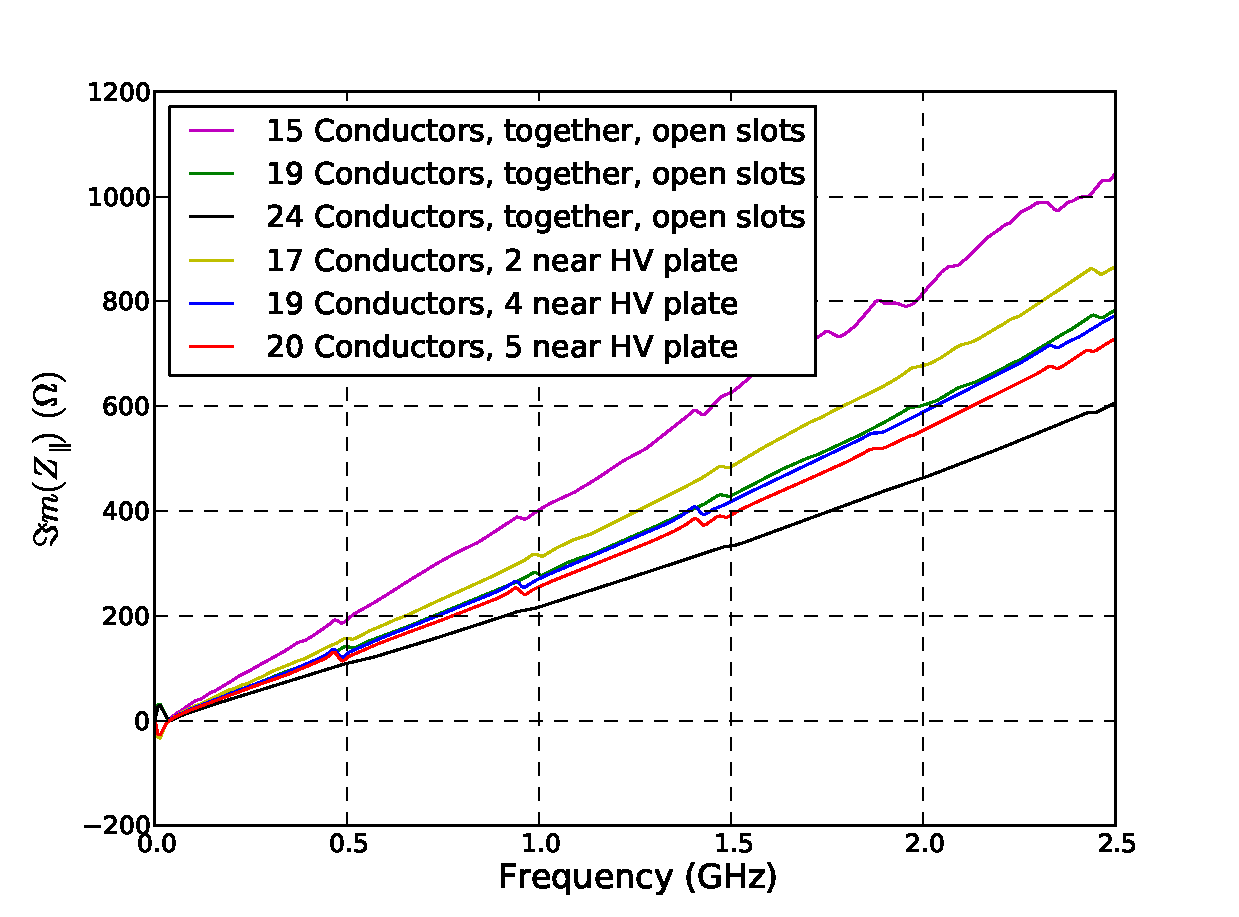
\includegraphics[width=0.5\textwidth]{LHC_MKI/figures/mki-no-screen-conductors-imag-impedance.pdf}
\label{fig:remove-cond-imag-imp}
}

\label{fig:remove-cond-impedance}
\caption{The longitudinal impedance of the MKIs with different numbers of screen conductors included in the beam screen. Shown is the real component \ref{fig:remove-cond-real-imp} and the imaginary component \ref{fig:remove-cond-imag-imp} of the longitudinal impedance.}
\end{figure}

The longitudinal impedance for these configurations is shown in Fig.~\ref{fig:remove-cond-impedance}. It can be seen that for both components of the impedance that more screen conductors reduces the magnitude of the impedance at all frequencies - this can simply be understood as improving the screening of the beam from the ferrite with additional screen conductors. This can particularly be seen in the increase in the number of screen conductors from 15 to 19 to 24 conductors in total - The screening is improved dramatically in each subsequent case. This also translates into a decrease in the expected beam-induced power loss in the structure, as shown in Tab.~\ref{tab:power-loss-cond-removal}. 

In addition it can be seen that it is preferable to distribute the screen conductors such that the maximum arc of the beam screen without screen conductors is minimised. This can clearly be seen by comparing the case of 19 screen conductors where all conductors are clustered together (as was done for the replacement MKI8d) and for 19 screen conductors, where 4 are equally distributed towards the HV busbar. Again this advantage is bourne out in the power lost in the structure. This is however not beneficial without consideration of the induced electric field during kicker firing, as the induced voltage on a given screen conductor is still the same, and thus tracking along the beam screen to the external metallization is not changed by this layout. It can thus be seen that the beam screen design itself must be optmised with regards to the induced screen conductor voltage before more can be added to the ceramic tube to improve screening.

\begin{table}
\label{tab:power-loss-cond-removal}
\begin{center}
\begin{tabular}{c | c | c}
Screen Conductor Arrangement & $P_{loss, BB}$ & $P_{loss, Res}$ \\ \hline
15 Conductors, together & $P_{loss, BB}$ & $P_{loss, Res}$ \\ \hline
19 Conductors, together & $P_{loss, BB}$ & $P_{loss, Res}$ \\ \hline
24 Conductors, together & $P_{loss, BB}$ & $P_{loss, Res}$ \\ \hline
17 Conductors, separated & $P_{loss, BB}$ & $P_{loss, Res}$ \\ \hline
19 Conductors, seperated & $P_{loss, BB}$ & $P_{loss, Res}$ \\ \hline
20 Conductors, seperated & $P_{loss, BB}$ & $P_{loss, Res}$ \\ \hline
\end{tabular}
\end{center}
\end{table}

\subsection{Dependence of the Impedance on the Beam Screen Dimensions}

It can be seen that with 24 screen conductors placed in the beam screen that the resulting impedance is dominated by the configuration of the beam screen. To investigate how changes to certain parameters (specifically the length of the overlap between the screen conductors and the external metallization and the thickness of the ceramic beam screen) a cut down model of the kicker magnet is used, considering just the capactively coupled end of the kicker magnet (shown in Fig.~\ref{fig:cut-down-mki-cap-end}). This is done to allow a larger mesh density in this important (from the electrical and impedance point of view) region of the kicker magnet. In models of the full kicker magnet the mesh density is severely limited due to the large mesh generated in the entire magnet volume which subsequently may make the mesh very limited in near beam areas (for example in the ceramic tube between the screen conductors and the external metallization. A comparison is shown in Fig.~\ref{fig:mki-mesh-com-cst}). An illustrated diagram of the capacitively coupled end is given in Fig.~\ref{fig:cap-end-diag} to clarify the components referred to in this section.

\begin{figure}
\subfigure[]{
\label{fig:cut-down-mki-cap-end}
}
\subfigure[]{
\label{fig:cap-end-diag}
}
\caption{\ref{fig:cut-down-mki-cap-end} The cut down simulation model used for simulations of the MKI beam screen with 24 screen conductors and \ref{fig:cap-end-diag} an illustrated diagram of the capacitively coupled end of the beam screen.}
\end{figure}

\begin{figure}
\subfigure[]{
\label{fig:mesh-full}
}
\subfigure[]{
\label{fig:mesh-cutdown}
}
\label{fig:mki-mesh-com-cst}
\caption{A comparison of the mesh that may be generated in CST Particle Studio using both the full model \ref{fig:mesh-full} and the cutdown model \ref{fig:mesh-cutdown}. Blue squares reresent a meshing failure which inserts perfect electrical conductor into the model. The simulation time for the first is on the order a day, for the second 30 minutes.}
\end{figure}